\documentclass[10pt]{beamer}

\usetheme{metropolis}
\usepackage{appendixnumberbeamer}

\usepackage{booktabs}
\usepackage[scale=2]{ccicons}

\usepackage{pgfplots}
\usepgfplotslibrary{dateplot}

\usepackage{xspace}
\newcommand{\themename}{\textbf{\textsc{metropolis}}\xspace}

\graphicspath{{graphics/}}

\title{Trump + President = Shakedown}
\subtitle{Measuring Ideological Differences with Word Embeddings}
\date{\today}
\author{Mike Burnham \\ mlb6496@psu.edu \\ github.com/MLBurnham/word\_embeddings}
\institute{Penn State University}
% \titlegraphic{\hfill
\includegraphics[height=1.5cm]{logo.pdf}}

\begin{document}

\maketitle

\begin{frame}{Table of contents}
  \setbeamertemplate{section in toc}[sections numbered]
  \tableofcontents[hideallsubsections]
\end{frame}

%%%%%%%%%%%%%%%%%%%%%%%%%%
% Introduction
%%%%%%%%%%%%%%%%%%%%%%%%%%

\section{Introduction}

\begin{frame}[fragile]{Background}
  Two dominant methods in this space:
  \begin{enumerate}
      \item Dictionary methods
        \begin{itemize}
            \item Inherently noisy
        \end{itemize}{}
      \item Sentiment analysis
        \begin{itemize}
            \item Lacks context
        \end{itemize}{}
  \end{enumerate}{}
  \bigskip
  Word embeddings were invented in 2013 and alleviate both of these problems. However, their use has almost exclusively been limited to predictive rather than explanatory applications
\end{frame}

%%%%%%%%%%%%%%%%%%%%%%%%%%%%%
% Background and lit review
%%%%%%%%%%%%%%%%%%%%%%%%%%%%%

\section{Background and Lit Review}

\begin{frame}{What is a word embedding?}
Word embeddings are language models that represent words as vectors of numbers. Those vectors are defined by the other words surrounding that word. Two important implications for this research:
  \begin{enumerate}
      \item This allows us to do math with words  
      \item Word vectors are not universal
  \end{enumerate}  
  \textbf{Distributional Hypothesis:} Words that appear in the same context tend to have similar meaning
\end{frame}

\begin{frame}{What is a word embedding? Example}
        \centering
        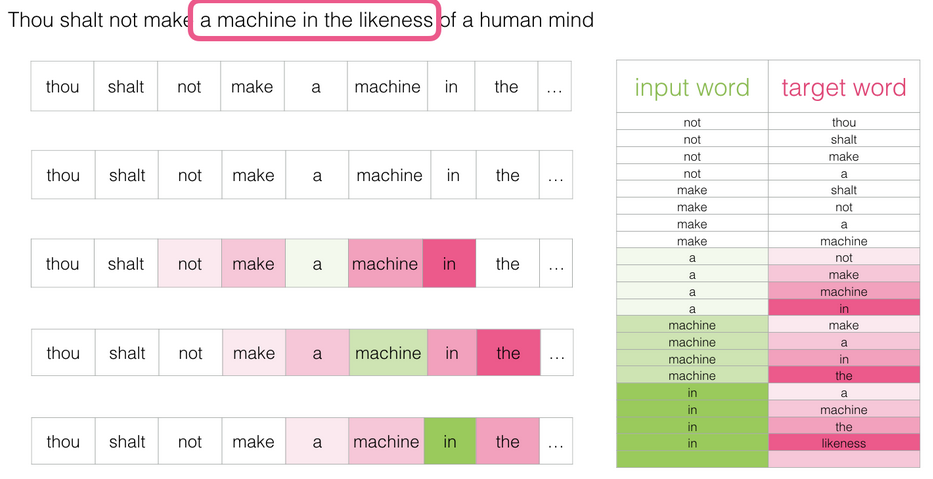
\includegraphics[width=1\textwidth]{embeddings_explained.png}
        \cite{word2vec}
\end{frame}

\begin{frame}{What is a word embedding? Example}
    
\includegraphics[width=.475\textwidth]{popkins.jpg}
    =
    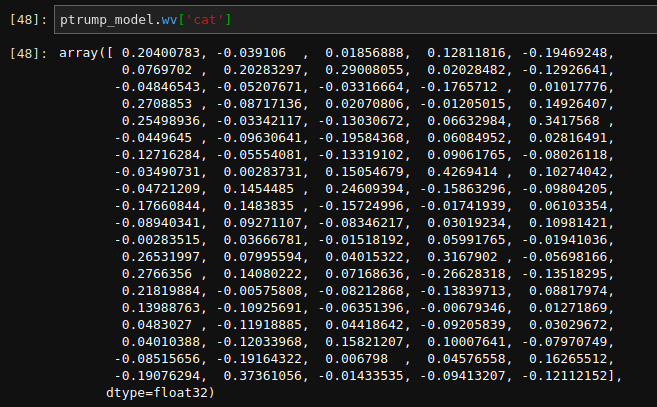
\includegraphics[width=.475\textwidth]{cat}
\end{frame}

\begin{frame}{What is a word embedding? Example}
  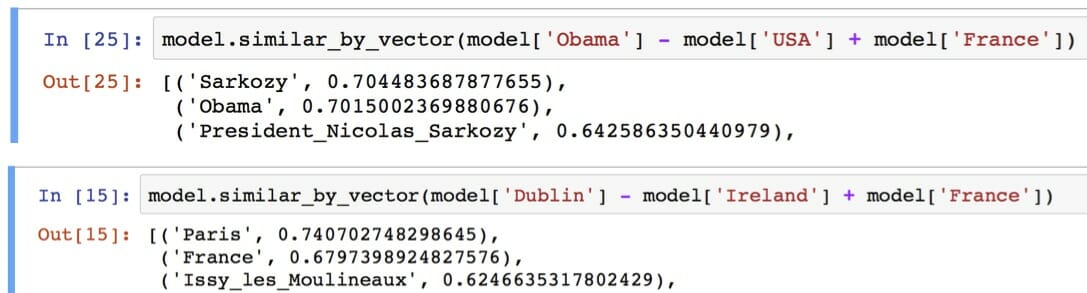
\includegraphics[width=1\textwidth]{vectormath1.jpg}
  \cite{word2vec}
\end{frame}

\begin{frame}{What is a word embedding? Example}
  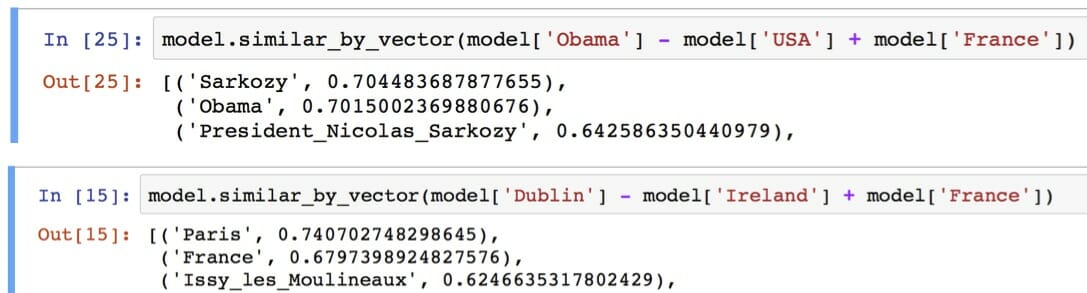
\includegraphics[width=1\textwidth]{vectormath1.jpg}
  \cite{word2vec}
  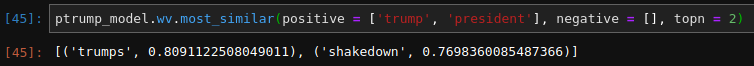
\includegraphics[width=1\textwidth]{trump_math.png}
\end{frame}

\begin{frame}{Literature: Diachronic Word Embeddings}
  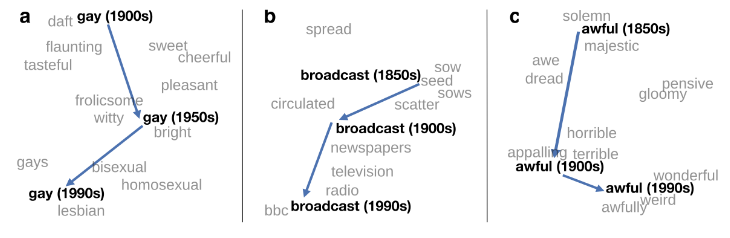
\includegraphics[width=1\textwidth]{diachronic.png}
  \cite{diachronic}
\end{frame}

\begin{frame}{Literature: Words are Malleable}
  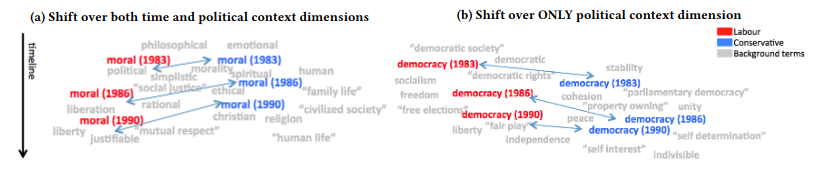
\includegraphics[width=1\textwidth]{malleable.png}
  \cite{malleable}
\end{frame}

\begin{frame}{Questions}
  \begin{enumerate}
      \item Can word embeddings capture the qualitative dimensions of political positions?
      \item Can word embeddings capture the quantitative dimensions of political positions?
      \item If so, what is the most effective implementation?
  \end{enumerate}    
\end{frame}

\begin{frame}{Questions}
  \begin{enumerate}
      \item Can word embeddings capture the qualitative dimensions of political positions? \textbf{Yes}
      \item Can word embeddings capture the quantitative dimensions of political positions?
      \item If so, what is the most effective implementation?
  \end{enumerate}    
\end{frame}

\begin{frame}{Questions}
  \begin{enumerate}
      \item Can word embeddings capture the qualitative dimensions of political positions? \textbf{Yes}
      \item Can word embeddings capture the quantitative dimensions of political positions? \textbf{Maybe}
      \item If so, what is the most effective implementation?
  \end{enumerate}    
\end{frame}

\begin{frame}{Questions}
  \begin{enumerate}
      \item Can word embeddings capture the qualitative dimensions of political positions? \textbf{Yes}
      \item Can word embeddings capture the quantitative dimensions of political positions? \textbf{Maybe}
      \item If so, what is the most effective implementation? \textbf{Unknown}
  \end{enumerate}
  This research re-examines the first two questions, and explores a new implementation by comparing word vectors within a single vector space, rather than across vector spaces.
\end{frame}

%%%%%%%%%%%
% Research Design
%%%%%%%%%%%
\section{Research Design}

\begin{frame}{Hypotheses}
    \begin{enumerate}
        \item A word that represents a political division between democrats and republicans will have a lower cosine similarity with its counterpart than a word that represents agreement.
        \item The words in closest proximity to divisive words will highlight points of contention 		between groups. 
    \end{enumerate}
\end{frame}

\begin{frame}{Process}
    \begin{enumerate}
        \item Collect Data
        \item Identify key words and their synonyms
        \item Pre-process text
        \item Train embeddings
        \item Analyze results
    \end{enumerate}{}
\end{frame}

\begin{frame}{1. Collect Data}
  \begin{itemize}
      \item Data should have a clear division between ideological groups and present clear ideological stances
      \item All tweets from Democratic or Republican Congress members between 11/06 and 12/10
  \end{itemize}
    \begin{figure}
        \centering
        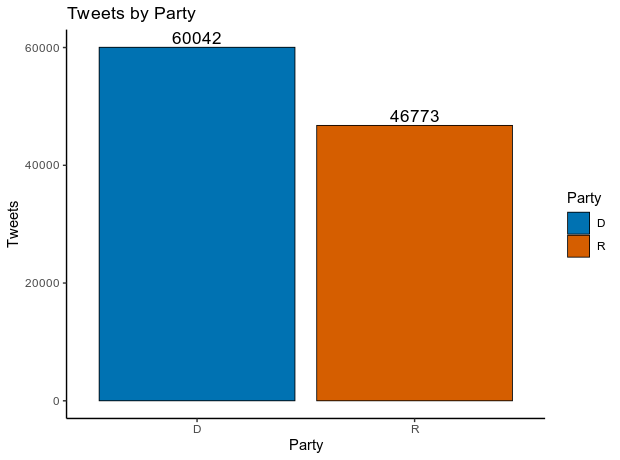
\includegraphics[scale=.5]{tweetcount}
    \end{figure}
\end{frame}

\begin{frame}{2. Identify Keywords}
    There types of keywords: disagree, agree, and baseline. \\
    Good keywords have three qualities:
    \begin{enumerate}
        \item Represent a clear point of (dis)agreement with well formulated positions. 
        \item Have a high usage
        \item Have an unambiguous interpretation and narrow context
    \end{enumerate}
    E.g. Impeachment is a good keyword, healthcare is not. 
    
    \begin{table}[]
        \centering
        \begin{tabular}{123}
        \toprule
          Label & n & Examples\\
          \midrule
          Disagree & 30 & trump, abortion, gun\\
          Agree & 8 & veteran, isis, infrastructure\\
          Base & 53 & answer, opportunity, member\\
          \bottomrule
        \end{tabular}
        \caption{Key Words}
        \label{tab:my_label}
    \end{table}{}
    
\end{frame}
\begin{frame}{3. Pre-process text}
  \begin{itemize}
      \item Remove punctuation, emoji, digits. Convert everything to lower case.
      \item Remove stopwords based on a modified version of spaCy's stopwords list
      \item Isolate and tag key word of interest
      \item Lemmatize text using spaCy's small english language model
  \end{itemize}
\end{frame}

\begin{frame}{4. Train embeddings}
\begin{itemize}
    \item A new embedding is trained for each key word
    \item Used Gensim's Word2vec implementation 
    \begin{itemize}
        \item skip-gram architecture
        \item 100 dimensions
        \item window size = 10
        \item learning rate = .025
    \end{itemize}
\end{itemize}
    
\end{frame}


%%%%%%%%%%%%%%%
% Results
%%%%%%%%%%%%%%%
\section{Results}

\begin{frame}{Distribution}
   \begin{table}
    \caption{Cosine similarity distribution}
    \begin{tabular}{12345}
      \toprule
      Label & Mean & Min & Max & n\\
      \midrule
      Disagree & 0.59 & 0.28 & 0.82 & 30\\
      Agree & 0.77 & 0.68 & 0.84 & 8\\
      Base & 0.63 & 0.41 & 0.86 & 53\\
      \bottomrule
    \end{tabular}
  \end{table}

  \begin{figure}
    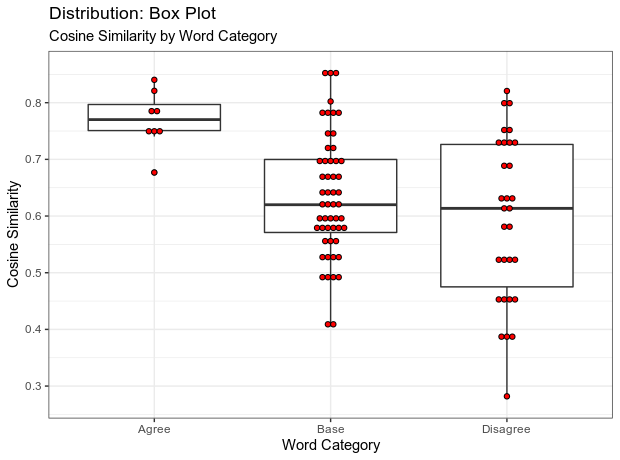
\includegraphics[width=.475\textwidth]{boxplot}
    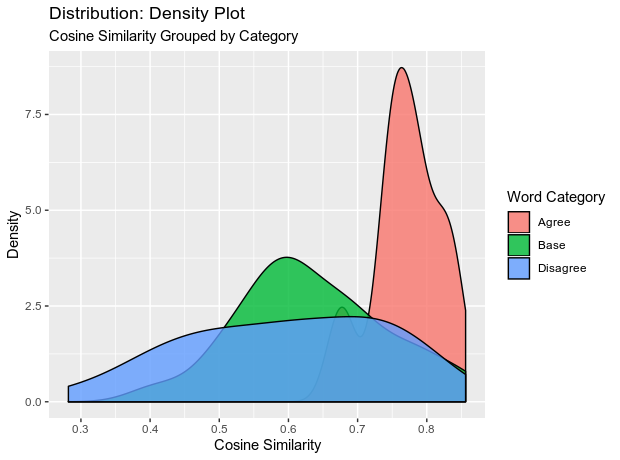
\includegraphics[width=.475\textwidth]{density}
  \end{figure}
\end{frame}

\begin{frame}{Significance Tests: All Words}
    \begin{figure}
        \centering
        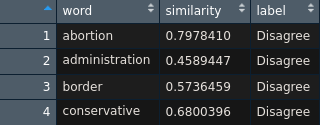
\includegraphics[width=.5\textwidth]{data1.png}
    \end{figure}
    
     \begin{table}
    \caption{Difference of means relative to disagree words}
    \begin{tabular}{12345678}
      \toprule
      Label    & Mean  & t-test (p) & Permutation (p) & Bootstrap (CI)\\
      \midrule
      Disagree & 0.59  & -          & -               & -\\
      Agree    & 0.77  & 2.11e-05   & 0.002           & (-0.27, -0.13)\\
      Base     & 0.63  & 0.29       & 0.23            & (-0.09, 0.02)\\
      \bottomrule
    \end{tabular}
  \end{table}

\end{frame}

\begin{frame}{Significance Tests: Trump}
    Observed value: 0.38 \\
    Mean permutation value: 0.87 \\
    Min permutation value: 0.80 \\
    p-value: 0.0 
    
    \begin{figure}
        \centering
        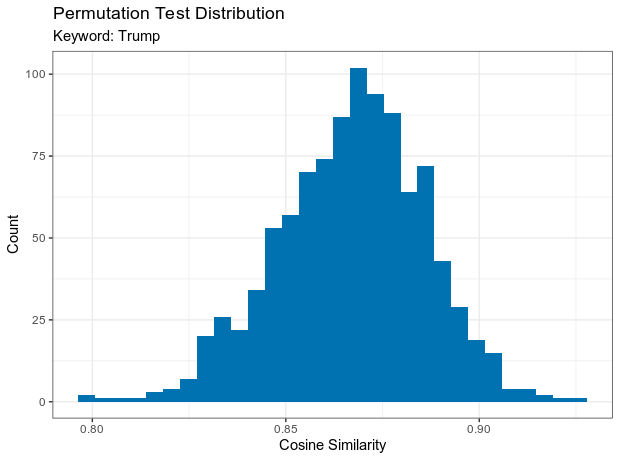
\includegraphics[width=.75\textwidth]{permutation.png}
    \end{figure}
\end{frame}

\begin{frame}{Qualitative Tests: Impeach}
      \begin{figure}
    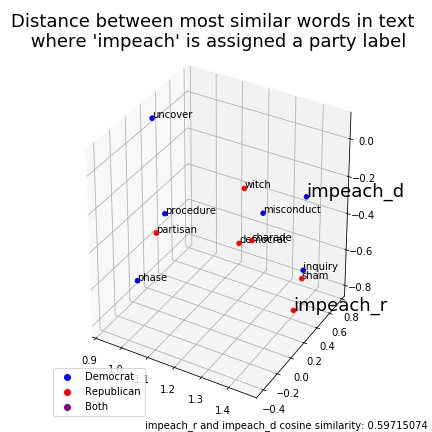
\includegraphics[width=.475\textwidth]{impeach_party.png}
    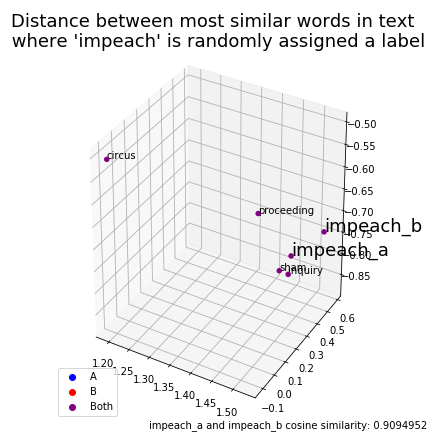
\includegraphics[width=.475\textwidth]{impeach_random.png}
  \end{figure}
\end{frame}

%%%%%%%%%%%%%%
% Conclusion
%%%%%%%%%%%%%%

\section{Conclusion}

\begin{frame}{Next Steps}
    \begin{itemize}
        \item Compare results with alternative methods, (Procrustes, fightin words)
        \item Test on a larger and more suitable data set (troll tweets?)
        \item Introduce new dimensions for capturing disagreement (sentiment)
        \item If successful, build a generalizable pipeline
    \end{itemize}
\end{frame}

%%%%%%%%%%%%%%
% Bibliography
%%%%%%%%%%%%%%

\begin{frame}{Bibliography}
  \begin{thebibliography}{}
    \bibitem{word2vec}
    Jay Alammar
    \textit{The Illustrated Word2vec}
    http://jalammar.github.io/illustrated-word2vec/
    
    \bibitem{diachronic}
      William L. Hamilton, Jure Leskovec, Dan Jurafsky
      \textit{Diachronic Word Embeddings Reveal Statistical Laws ofSemantic Change}
       arXiv preprint arXiv:1605.09096 (2016).
    
    \bibitem{malleable}
    Hosein Azarbonyad, Mostafa Dehghani, Kaspar Beelen, Alexandra Arkut, Maarten Marx, Jaap Kamps
    \textit{Words are Malleable: Computing Semantic Shifts in Political and Media Discourse}
    In Proceedings of the 2017 ACM on Conference on Information and Knowledge Management, pp. 1509-1518. ACM, 2017.
    
  \end{thebibliography} 
\end{frame}


\end{document}
